\documentclass[12pt,a4paper]{article}

\usepackage[margin=0.9in]{geometry}
\usepackage{amsmath,amssymb}
\usepackage{booktabs}
\usepackage{tabularx}
\usepackage{enumitem}
\usepackage{hyperref}
\usepackage{xcolor}
\usepackage{fancyhdr}
\usepackage{caption}
\usepackage{tikz}
\usepackage{tcolorbox}

\usetikzlibrary{arrows.meta,positioning,calc}
\tcbuselibrary{skins,breakable}

% Neutral palette for formal academic presentation
\definecolor{primary}{RGB}{0,0,0}
\definecolor{secondary}{RGB}{60,60,60}
\definecolor{accent}{RGB}{85,85,85}
\definecolor{highlight}{RGB}{110,110,110}
\definecolor{danger}{RGB}{140,140,140}
\definecolor{light}{RGB}{245,245,245}

\hypersetup{
    hidelinks,
    pdftitle={Explained, Unexplained, and Total Deviation in Simple Linear Regression},
    pdfauthor={Department of Computing}
}

\pagestyle{fancy}
\fancyhf{}
\lhead{Simple Linear Regression}
\rhead{Deviation Decomposition Report}
\rfoot{Page \thepage}

\setlength{\parskip}{0.5em}
\setlength{\parindent}{0pt}
\setlength{\headheight}{15pt}

\newtcolorbox{defbox}[1]{
    colback=primary!5,
    colframe=primary,
    title=#1,
    fonttitle=\bfseries,
    rounded corners,
    boxrule=0.9pt,
    breakable
}

\newtcolorbox{insightbox}{
    colback=accent!8,
    colframe=accent,
    title=Key Insight,
    fonttitle=\bfseries,
    rounded corners,
    boxrule=0.9pt,
    breakable
}

\newtcolorbox{warningbox}{
    colback=highlight!10,
    colframe=highlight,
    title=Common Pitfall,
    fonttitle=\bfseries,
    rounded corners,
    boxrule=0.9pt,
    breakable
}

\begin{document}

\begin{titlepage}
\centering
\vspace*{0.5cm}
{\Large\color{primary}\textbf{Academic Analytical Report}}\\[0.3cm]
\rule{\textwidth}{1.8pt}\\[0.5cm]
{\Huge\bfseries\color{primary}Explained, Unexplained, and Total Deviation}\\[0.2cm]
{\Large In Simple Linear Regression}\\[0.4cm]
\rule{\textwidth}{1.8pt}\\[1.0cm]

\begin{tabular}{rl}
\textbf{Model Type:} & Simple Linear Regression \\
\textbf{Focus:} & Deviation decomposition and variance interpretation \\
\textbf{Core Terms:} & Total Deviation, Explained Deviation, Residual Deviation \\
\textbf{Output:} & Mathematical and visual explanation with worked example
\end{tabular}

\vfill
{\large Department of Computing}\\
{\large \today}
\end{titlepage}

\tableofcontents
\newpage

\section{Introduction}

In simple linear regression, we predict a response variable $y$ from one predictor $x$ using the fitted line
\begin{equation}
\hat{y}_i = b_0 + b_1 x_i.
\end{equation}

A central question is: \textit{how much of the variation in $y$ is captured by the regression line, and how much remains as error?}

This is answered by decomposing deviations into three parts:
\begin{itemize}[noitemsep]
    \item \textbf{Total deviation} from the overall mean,
    \item \textbf{Explained deviation} due to the fitted line,
    \item \textbf{Unexplained deviation} (residual error).
\end{itemize}

\section{Core Definitions}

Let $\bar{y}$ be the sample mean of observed responses.

\begin{defbox}{Deviation Terms for Observation $i$}
\textbf{1) Total deviation}
\begin{equation}
\text{Total}_i = y_i - \bar{y}
\end{equation}
This measures how far the actual value is from the overall average.

\textbf{2) Explained deviation}
\begin{equation}
\text{Explained}_i = \hat{y}_i - \bar{y}
\end{equation}
This is the part of deviation captured by the regression model.

\textbf{3) Unexplained deviation (residual)}
\begin{equation}
\text{Unexplained}_i = y_i - \hat{y}_i = e_i
\end{equation}
This is the remaining error not explained by the model.
\end{defbox}

For every data point, the additive identity is:
\begin{equation}
\underbrace{(y_i-\bar{y})}_{\text{Total}} =
\underbrace{(\hat{y}_i-\bar{y})}_{\text{Explained}} +
\underbrace{(y_i-\hat{y}_i)}_{\text{Unexplained}}.
\label{eq:pointwise}
\end{equation}

\section{Diagram: Pointwise Decomposition}

Figure~\ref{fig:pointwise} shows the same vertical distance split into two pieces.

\begin{center}
\resizebox{0.95\textwidth}{!}{%
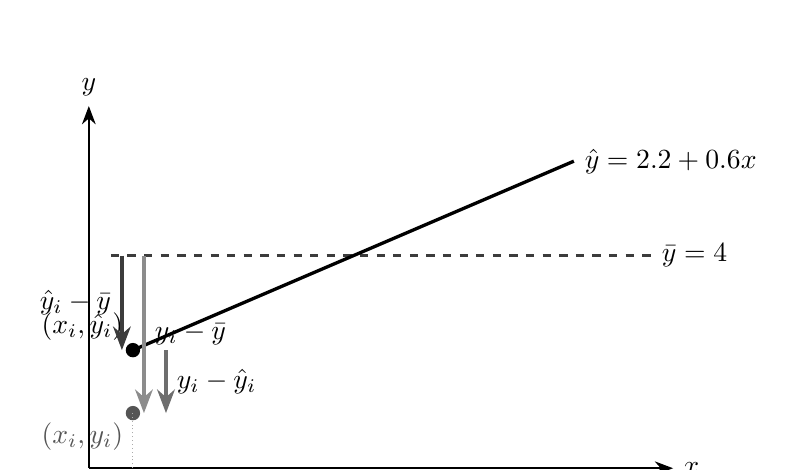
\begin{tikzpicture}[x=1.4cm,y=1.0cm,>=Stealth]

    % Axes
    \draw[->,thick] (0.6,1.3) -- (5.9,1.3) node[right] {$x$};
    \draw[->,thick] (0.6,1.3) -- (0.6,5.9) node[above] {$y$};

    % Mean line and regression line
    \draw[secondary,dashed,very thick] (0.8,4.0) -- (5.7,4.0) node[right,black] {$\bar{y}=4$};
    \draw[primary,very thick] (1.0,2.8) -- (5.0,5.2) node[right,black] {$\hat{y}=2.2+0.6x$};

    % Data points
    \fill[accent] (1.0,2.0) circle (2.6pt) node[below left] {$\,(x_i,y_i)$};
    \fill[primary] (1.0,2.8) circle (2.6pt) node[above left] {$\,(x_i,\hat{y}_i)$};

    % Deviation arrows
    \draw[danger,very thick,-{Stealth[length=3mm]}] (1.10,4.0) -- (1.10,2.0)
        node[midway,right,black] {$y_i-\bar{y}$};

    \draw[secondary,very thick,-{Stealth[length=3mm]}] (0.90,4.0) -- (0.90,2.8)
        node[midway,left,black] {$\hat{y}_i-\bar{y}$};

    \draw[highlight,very thick,-{Stealth[length=3mm]}] (1.30,2.8) -- (1.30,2.0)
        node[midway,right,black] {$y_i-\hat{y}_i$};

    % Visual guide
    \draw[light!70!black,densely dotted] (1.0,1.3) -- (1.0,2.0);

\end{tikzpicture}
}
\captionof{figure}{Pointwise decomposition: total deviation = explained deviation + unexplained deviation.}
\label{fig:pointwise}
\end{center}

\begin{insightbox}
Equation~\eqref{eq:pointwise} holds for each point. In words: from mean to actual value equals from mean to prediction plus from prediction to actual value.
\end{insightbox}

\section{From Deviations to Sums of Squares}

To measure variation for the \textit{entire dataset}, square and sum the deviations:
\begin{align}
\text{SST} &= \sum_{i=1}^{n}(y_i-\bar{y})^2 \quad \text{(Total Sum of Squares)} \\
\text{SSR} &= \sum_{i=1}^{n}(\hat{y}_i-\bar{y})^2 \quad \text{(Regression/Explained Sum of Squares)} \\
\text{SSE} &= \sum_{i=1}^{n}(y_i-\hat{y}_i)^2 \quad \text{(Error/Residual Sum of Squares)}
\end{align}

For ordinary least squares with an intercept term,
\begin{equation}
\text{SST} = \text{SSR} + \text{SSE}.
\label{eq:sstsplit}
\end{equation}

\begin{defbox}{Why Equation~\eqref{eq:sstsplit} Works}
Expanding $(y_i-\bar{y}) = (\hat{y}_i-\bar{y}) + (y_i-\hat{y}_i)$ and summing squares creates a cross-term:
\begin{equation}
2\sum_{i=1}^{n}(\hat{y}_i-\bar{y})(y_i-\hat{y}_i).
\end{equation}
In OLS with intercept, fitted values and residuals are orthogonal, so this cross-term is zero. Therefore, the variance partition is exact.
\end{defbox}

\section{Diagram: Variance Partition Pipeline}

\begin{center}
\resizebox{0.95\textwidth}{!}{%
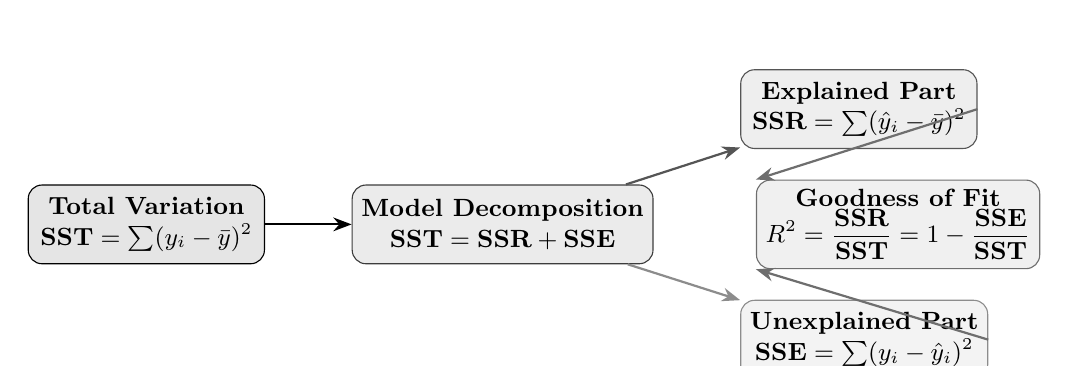
\begin{tikzpicture}[
    node distance=0.7cm,
    box/.style={rectangle,rounded corners=5pt,draw=#1,fill=#1!10,minimum width=3.0cm,minimum height=1.0cm,font=\small\bfseries,align=center},
    arrow/.style={-{Stealth},thick,#1}
]

\node[box=primary] (sst) {Total Variation\\$\text{SST}=\sum(y_i-\bar{y})^2$};
\node[box=secondary,right=1.1cm of sst] (split) {Model Decomposition\\$\text{SST}=\text{SSR}+\text{SSE}$};
\node[box=accent,above right=0.45cm and 1.1cm of split] (ssr) {Explained Part\\$\text{SSR}=\sum(\hat y_i-\bar y)^2$};
\node[box=danger,below right=0.45cm and 1.1cm of split] (sse) {Unexplained Part\\$\text{SSE}=\sum(y_i-\hat y_i)^2$};
\node[box=highlight,right=1.3cm of split] (r2) {Goodness of Fit\\$R^2=\dfrac{\text{SSR}}{\text{SST}}=1-\dfrac{\text{SSE}}{\text{SST}}$};

\draw[arrow=primary] (sst) -- (split);
\draw[arrow=accent] (split) -- (ssr);
\draw[arrow=danger] (split) -- (sse);
\draw[arrow=highlight] (ssr.east) -- (r2.north west);
\draw[arrow=highlight] (sse.east) -- (r2.south west);

\end{tikzpicture}
}
\captionof{figure}{Total variation is split into explained and unexplained components, which define $R^2$.}
\label{fig:pipeline}
\end{center}

\section{Worked Numerical Example}

Consider the dataset:
\begin{center}
$ (x,y) = (1,2),(2,4),(3,5),(4,4),(5,5) $
\end{center}

The fitted simple linear regression line is:
\begin{equation}
\hat{y} = 2.2 + 0.6x,
\end{equation}
with mean response $\bar{y}=4$.

\begin{center}
\small
\begin{tabular}{cccccccc}
\toprule
$i$ & $x_i$ & $y_i$ & $\hat y_i$ & $y_i-\bar y$ & $\hat y_i-\bar y$ & $y_i-\hat y_i$ & Squares Contribution \\
\midrule
1 & 1 & 2 & 2.8 & -2.0 & -1.2 & -0.8 & $4.00,\ 1.44,\ 0.64$ \\
2 & 2 & 4 & 3.4 &  0.0 & -0.6 &  0.6 & $0.00,\ 0.36,\ 0.36$ \\
3 & 3 & 5 & 4.0 &  1.0 &  0.0 &  1.0 & $1.00,\ 0.00,\ 1.00$ \\
4 & 4 & 4 & 4.6 &  0.0 &  0.6 & -0.6 & $0.00,\ 0.36,\ 0.36$ \\
5 & 5 & 5 & 5.2 &  1.0 &  1.2 & -0.2 & $1.00,\ 1.44,\ 0.04$ \\
\midrule
\multicolumn{4}{r}{\textbf{Totals}} & & & &
$\textbf{SST}=6.00,\ \textbf{SSR}=3.60,\ \textbf{SSE}=2.40$ \\
\bottomrule
\end{tabular}
\end{center}

So the decomposition is exact:
\begin{equation}
6.00 = 3.60 + 2.40.
\end{equation}

And coefficient of determination is:
\begin{equation}
R^2 = \frac{\text{SSR}}{\text{SST}} = \frac{3.60}{6.00} = 0.60.
\end{equation}

Interpretation: \textbf{60\%} of total variation is explained by the regression line, and \textbf{40\%} remains unexplained.

\section{Interpretation Guide}

\begin{defbox}{How to Read Deviation Components}
\textbf{Large SSR, small SSE:} model captures most structure in data.\\
\textbf{Small SSR, large SSE:} predictor $x$ has weak linear explanatory power.\\
\textbf{High $R^2$:} strong in-sample fit (not always causality, not always best model).\\
\textbf{Low $R^2$:} weak linear fit; may still be useful in noisy domains.
\end{defbox}

\begin{warningbox}
$\text{SST}=\text{SSR}+\text{SSE}$ is guaranteed in ordinary least squares with an intercept. If the intercept is removed, this exact decomposition may not hold in the same form.
\end{warningbox}

\section{Conclusion}

In simple linear regression, total variation around the mean is partitioned into:
\begin{itemize}[noitemsep]
    \item explained variation due to the model, and
    \item unexplained variation due to residual errors.
\end{itemize}

This decomposition is the mathematical foundation behind the fit metric $R^2$ and offers a clear way to evaluate model quality both algebraically and graphically.

\end{document}
